\documentclass[journal]{./IEEEtran}
\usepackage{cite}
\usepackage[toc,page]{appendix}
\usepackage{graphicx}
\usepackage{amsmath}
\usepackage{algorithm}
\usepackage[noend]{algpseudocode}
\graphicspath{ {images/} }
\newcommand{\SPTITLE}{FactU: An Android Application for News Verification Using Sentence Similarity Analysis and Hidden Markov Model}
\newcommand{\ADVISEE}{Emmanuel B. Constantino Jr, Homer C. Malijan,}
\newcommand{\ADVISER}{Professor Caroline Natalie Peralta}

\newcommand{\BSCS}{Bachelor of Science in Computer Science}
\newcommand{\ICS}{Institute of Computer Science}
\newcommand{\UPLB}{University of the Philippines Los Ba\~{n}os}
\newcommand{\REMARK}{\thanks{Presented to the Faculty of the \ICS, \UPLB\
		in partial fulfillment of the requirements
		for the Degree of \BSCS}}

\markboth{CMSC 190 Special Problem, \ICS}{}
\title{\SPTITLE}
\author{\ADVISEE~and~\ADVISER%
	\REMARK
}
\pubid{\copyright~2017~ICS \UPLB}

%%%%%%%%%%%%%%%%%%%%%%%%%%%%%%%%%%%%%%%%%%%%%%%%%%%%%%%%%%%%%%%%%%%%%%%%%%

\begin{document}
    
	
	% TITLE
	\maketitle
	
	% ABSTRACT
	\begin{abstract}
		The Internet's ecosystem grows every second, and with it comes new information that might not be reliable or accurate. One of the biggest problems people face when surfing the Internet is information fabrication. Although possibly unintentional, the need to validate such statements is necessary. This paper presents an application that crawls through various reliable and satiric websites for information and matches statements to assess its validity. With over 5,000 news articles, a Hidden Markov Model (HMM) was used to structure relevant information depending on the user's input to be evaluated for its category: verified, satiric, or unverified.
	\end{abstract}
	
	% INDEX TERMS
	\begin{keywords}
		web crawler, natural language processing, fact validation, machine learning, hidden markov models, sentence similarity analysis
	\end{keywords}
	
	% INTRODUCTION
	\section{Introduction}
	As the literacy rate of the world increases, verification
	of information will be the next concern. The world is also
	starting to appreciate the World Wide Web, making it easier for people of any age bracket to surf for information on the Internet. This causes the Internet to be prone to hackers, trolls, or fake online information since most users believe what they see on the Internet.
	
	The study aims to verify a statement's validity by crawling
	through trusted and ''satiric'' web pages and comparing relevant articles, rating its resemblance and similarity, and use a Hidden Markov Model(HMM) to classify such input.
	
	\subsection{Significance of the Study}
	The inevitable growth of Internet users has made it a lot easier for information to spread in a short span of time. Not all information that is produced online can be reliable since all Internet users have the capability of reproducing and spreading information, especially on social media websites. This results in plenty of people acquiring questionable information which makes it harder for them to determine which information is legitimate. The study is relevant because of the increase in the number of hoax websites disseminating misleading information, especially in the field of politics and science.
	
	\subsection{Objective of the Study}
	The main purpose of the study is to develop an application
	that crawls the Internet for relevant information as a reference to classify input statements as verified, unverified, or satiric.
	
	Specifically, the study aims to achieve the following:
	
	\begin{itemize}
		\item To develop an Android application using Python that can help people verify statements that they see online using their smartphones, the same way dictionary applications are used to verify meaning of certain words;
		\item To crawl through various news websites to feed the database with information to better assess the user-defined statement;
		\item To evaluate whether or not a news article supports a particular statement using sentence similarity analysis; and
		\item To assess the effectiveness of using an HMM to classify news statements.
	\end{itemize}
	
	\subsection{Scope and Limitations of the Study}
    This study will focus on verifying news by analyzing data that was obtained from different trusted and satirical news websites. The range of the news from trusted news websites will be from local to international news. The information that will be gathered from these news websites will be evaluated through Sentence Similarity Analysis. These scores will be used to feed the HMM that will produce the final output.
    
    The computational model will greatly depend on the information gathered from various news websites. In essence, if a satiric website posts genuine news, the application will still label it as satiric because of its source.
    
    The application can only process statements that are not compound-complex sentences in structure to avoid inputs having multiple news contents. Moreover, news websites will only be crawled every 24 hours, meaning news may not be available as a source as soon as it is published. Lastly, this study is limited to news articles written in English.
	
	\section{Review of Related Literature}

	\subsection{Sentence Similarity Analysis}
	\pubidadjcol
	One of the crucial parts of this study is comparing various sentences and evaluating its similarity. There are many ways to measure the similarity between sentences. One method is through Word Overlapping, this is based on computing the number of exact words that can be seen in each sentence. Another method is through Linguistic Analysis. This method can be implemented in three different ways\cite{achananuparp}:
	
	\begin{enumerate}
		\item \emph{Semantic Textual Similarity}, combines Latent Semantic Analysis and Machine Learning algorithms;
		\item \emph{Word Order Similarity}, focuses on the measurement of basic syntactic information; the permutation of words; and
		\item \emph{Hybrid of Semantic and Syntactic similarity analysis}.
	\end{enumerate}
	
	A grammar approach is another way to calculate similarity. Using this approach, sentences are parsed to derive their grammatical structure \cite{lee14}.
	
	There are plenty of related studies in the field of Sentence Similarity Analysis. Research has been conducted to explore different methods in creating an Automated Short-Essay grading application. The app was intended to evaluate students' answers based on the correct answer given by the teacher.
	
	Measuring similarity is subjective but it can also be computed using different methods:
	
	\begin{enumerate}
		\item \emph{Euclidean Distance} is one of the most common metrics for measuring proximity; the closer the distance, the higher the similarity.		\item \emph{Manhattan Distance} is measured by getting the total sum of the difference between x-coordinates and y-coordinates.
		\item \emph{Minowski Distance} is a generalized method of getting distance. Both Euclidean and Manhattan Distance can be derived from it.
		\item \emph{Jaccard Similarity} is a method where objects are considered as sets. It simply gets the cardinality of the intersection of the sets divided by the cardinality of the union of the sets.
		\item \emph{Cosine Similarity} finds the cosine of the angle between the two objects (see Equation \ref{eq:cosinesimilarity}). It sees objects as vectors and computes for the normalized dot product. This similarity measure is used in this study. 
		
	    \begin{equation}
	        similarity = \frac{\sum_{i=1}^{n}A_i B_i}{\sqrt{\sum_{i=1}^{n}A_i^2} \sqrt{\sum_{i=1}^{n} B_i^2}}
	        \label{eq:cosinesimilarity}
	    \end{equation}
		
	\end{enumerate}
	
	\begin{figure}
		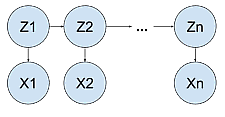
\includegraphics{trellis}
		\label{trellis}
		\caption{Illustration of a Hidden Markov Model.}
	\end{figure}
	
	% CNMP: If ASOBEK and MITRE stand for something, please spell them out.
	The ASOBEK system is a software application that aids in Sentence Similarity Analysis. It uses the Support Vector Machine (SVM) classification algorithm with the Word Overlapping method. On the other hand, the MITRE system uses Neural Networks with string matching features. Studies in the field of Sentence Similarity Analysis have greatly progressed in the past few years due to the increasing development of Artificial Intelligence. The growth can also be attributed to an annual competition named SemEval\cite{kashyap15}, where developers create systems that use Sentence Similarity Analysis based on a particular theme.
	
	\subsection{Web Crawler}
	Web Crawling is usually used in applications that require a wide array of data gathering procedures. These crawlers, typically called spiders, are deployed to websites where they recursively visit other links that may contain information about a topic of interest. Rahul Kamar, Anurag Jain, and Chetan Agrawal have surveyed a variety of web crawling algorithms \cite{kumar14} including Breadth First Search, Depth First Search, Page Rank Algorithm, Crawling Through URL Ordering, Batch-page Rank, Partial-page Rank, Using HTTP Get Request and Dynamic Web Pages, etc \cite{olston10}. All these algorithms further improve the performance of spiders because they usually run tedious processes and allocate a huge amount of information into a database for later computation.
	
	Since the Internet is a vast place, diverse algorithms have been developed to further amplify spiders' performance like skipping irrelevant web pages \cite{manku07} as described by Gurmeet Manku, Arvind Jain, and Anish Sarma. This greatly improved web crawlers' run time, ignoring ads and unrelated and malicious links. However, the technique is still in development because of the subjectivity in considering a link to be irrelevant to the topic of interest.
	
	Another factor that affects a web crawler's performance is keyword extraction as explained by Gunjan Agre and Nikita Mahajan \cite{agre15}. It can hasten a crawler's response as it does not require relevant feedback before it is considered to be a part of the training data. Rather, the crawler matches keywords from a certain topic with the keywords predefined within various web pages.
	
	Some crawlers that require parsing more than the Surface
	Web have also been developed by different programmers
	like that of Xiang Peisu, Tien Ke, and Huang Qinzhen. They developed an effective framework for Deep Web Crawling \cite{peisu08} that makes use of a number of novel techniques to scrape information from the Deep Web.
	
	\subsection{Python and Android}
	Python has been one of the most popular programming languages since its development in the late 1980’s by Guido van Rossum \cite{tulchak}. Today, Python is known to be an open-source, general-purpose scripting language. It is widely used and has a very wide array of libraries for various purposes.
	
	On the other hand, Android programming is hastily developing due to the recent smartphone revolution. 80\% of smartphones run in Android. There is a huge diversity of libraries to help programmers develop their own Android applications. 
	
	Due to both technologies' increasing popularity, libraries such as python-for-android were created. These libraries allow programmers to package Python code into standalone Android Packages (APKs) that can be copied or even uploaded to different marketplaces such as the Android Play Store \cite{kivy16}.
		
	\subsection{Hidden Markov Model}	
	The Hidden Markov Model (HMM) is one of the most popular models in Artificial Intelligence for sequential or temporal data. This model is simple, yet efficient in recuperating a series of states from a series of observations \cite{ramage13}. At present, HMMs are used in various speech recognition applications and numerous computational problems in molecular biology \cite{Ghahramani01}.
	
	HMMs are depicted in Fig. \ref{trellis}. Given $Z$, a finite sequence of discrete random variables, and $X$, finite sequence of values corresponding to each value in $Z$, ``hidden'' $Z$ values can be predicted using the observable values in $X$.
	
	\subsection{Related Work}
	
	\begin{figure}
		
\includegraphics{related}
		\label{related}
		\caption{Program flow of the Chrome browser extension by \cite{goel16}.}
	\end{figure}
	
	A group of four college students recently created a Chrome browser extension for a hackathon at Princeton University. They used Python 3.0 to verify links. Google Search was used to query the input and check if they are trustworthy based on a set of reliable websites \cite{goel16}. Their extension supports verifying Twitter screenshots as well. The program's flow is illustrated in Fig. \ref{related}. They use Google’s Tesseract OCR to extract the Tweet as well as the Twitter handle used to post the Tweet. They then query the Twitter handle online and open the matching profile. Each Tweet by the Twitter handle is parsed for a match with the text extracted from the screenshot \cite{bort16}. 
	
	% MATERIALS AND METHODS
	\section{Materials and Methods}
	
	FactU was implemented using Python 3, and is compatible with Android 5.0 or later. It takes a simple sentence or Uniform Resource Locator (URL) to verify, and queries its database for related news articles that were found during the web crawling process. It then determines whether the input is backed up by verified (credible) or satiric news sources or if it is unverified, that is, there is not enough evidence to classify it as verified or satiric.
	
	Specify all libraries used with brief descriptions here.
	
	\subsection{Web Crawling and Database}
	The application made use of an SQLite3 database for a simple implementation of a database in terms of Python. It also has a Graphical User Interface (GUI) that makes it easier to monitor stored data. It also makes information migration easier since it generates a database file which can be copied from different systems.
	
	The web crawler deploys a spider to the home page of each news website (see Table \ref{tablea}), both credible and satiric. This spider visits every link in the current page and exhausts every link recursively to try to take the title, author, publish date, body of the news, as well as the URL. All information is  stored in the database. The spider was not able to get the author and publish dates of some websites since some articles follow a different HTML structure. These columns are left blank to prevent the processing of faulty information.
	
	A script was used to linearly deploy all spiders and maintain the database at the same time. The script contains a loop that re-runs the same process every 24 hours to catch new information on every concerned website's home page.
	
	\begin{table}[h!]
	       \caption{List of Reliable and Satiric websites}
	    \begin{center}
    		\begin{tabular}{ |c|c| } 
    			\hline
    			Reliable Websites & Satiric Websites \\ 
    			\hline
    			http://www.aljazeera.com/ & https://adobochronicles.com/  \\ 
    			http://www.bbc.com/news & http://www.newsbiscuit.com/  \\ 
    			http://edition.cnn.com/ & Dailycurrant.com  \\ 
    			http://www.foxnews.com/ & theonion.com  \\ 
    			https://news.google.com/ & http://www.socialnewsph.com/  \\ 
    			https://www.theguardian.com  & \\ 
    			http://www.nbcnews.com/  & \\ 
    			\hline
    		\end{tabular}
    		
    		\label{tablea}
    	\end{center}	
    \end{table}	
	

	\subsection{Sentence Similarity Analysis}
	Latent Semantic Analysis (LSA) is a method used for analyzing the relationship between terms and statements which will be used in retrieving similar sentences. The platform used to implement LSA was the Natural Language Toolkit (NLTK).
	
	NLTK is one of the most popular packages used in natural language processing. The  package includes Wordnet, a lexical database that can be used to determine word definitions, synonyms, homonyms, and to identify parts of speech.
	
	The list of news articles relevant to the user's input are retrieved from the database maintained by the web crawler, and each article's similarity to the input is computed. Each sentence is preprocessed before computing similarity by tokenization and parts-of-speech identification. The BLLIP parser was also used in this study to determine the syntactic structure of the string. The process of computing sentence similarity is shown in Fig. \ref{ssa}.
	
	After processing each word in the string, three different approaches were used to calculate Semantic Similarity.
	
	\subsubsection{Triplet Extraction Approach}
	
	This approach was derived from the paper of Yuntong Liu and Yanjun Liang about calculating Sentence Semantic Similarity based on Segmented Semantic Comparison\cite{yuntong13}. Triplet extraction tracks the subject, verb, and object (SVO) of a sentence. The idea is to get the SVO of the sentences and compare each segment to its corresponding segment in the other sentences. Cosine Similarity is used for computing the semantic relationship between each set of SVOs. Lastly, Wu-Palmer Similarity, which shows how similar two-word senses are based on the depth of the senses in the taxonomy, for computing the semantic relationship between each word.
	
	The syntactic structure produced by the BLLIP parser was used to get the SVO of the sentence. The set of nouns found in the first Noun Phrase (NP) is considered the subject of the sentence. The deepest verb found in the Verb Phrase (VP) subtree before encountering a Noun Phrase, Prepositional Phrase (PP) or an Adjective Phrase (ADJP) is considered the verb of the sentence. Lastly, nouns and adjectives encountered in the last subtrees are the objects of the sentence. Proper nouns that are consecutively placed in the sentence are automatically merged. After getting the SVO of each sentence, the segments are converted to vector space in order to compute the Cosine Similarity. Each word is compared to other words using Wu-Palmer Similarity. After getting each score from each segment, coefficients are used to weigh each segment. The sum of each segment multiplied to its corresponding coefficient is the final similarity score of the two sentences.
	
	\subsubsection{NV-Space Approach}
	This approach was implemented based on the paper of Ming Che Lee, Jia Wei Zhang, Wen Xiang Lee, and Heng Yu Ye on Sentence Similarity Computation based on Parts-of-Speech and Semantic Nets \cite{lee09}. All of the nouns and verbs of each sentence are identified to form a noun and verb set. Each set is compared to its corresponding set in other sentences.
	
	This approach also uses Cosine Similarity in order to get the Noun Cosine and the Verb Cosine. Wu-Palmer Similarity was also used for getting the relationship between each word. The proposed coefficients to be used were 0.65 and 0.35 for the Noun Cosine and Verb Cosine, respectively.
	
	\subsubsection{Semantic and Word Order Similarity Approach}
	Yuhua Li, Zuhair Bandar, David McLean and James O’Shea conducted a study about measuring Sentence Similarity for Short Sentences \cite{lee}. A vector space for both sentences is created the shortest path length between words is measured to get the similarity. It also considers Word Order Similarity, since placing words in a different order may result in different meanings. Coefficients were also used for weighing the Semantic Similarity and the Word Order Similarity. Adding the two similarities would result in the final similarity score.
	
	Similarity scores using these approaches were computed and used for the HMM in order to verify the user's input.
	
	\begin{figure}
		
\includegraphics{ssa}
		\caption{Sentence Similarity Analysis flow chart.}
		\label{ssa}
	\end{figure}
	
	\subsection{Hidden Markov Model}
	The model is constructed using the similarity scores received from the Sentence Similarity Analysis module as to a set of sentences, Z, formed like a Markov Chain with a corresponding pairing with the type of website, X, it came from, either reliable or satiric. The states in this study are Verified, Satiric and Not Verified. However, only the Verified and Satiric states were used for the HMM because Not Verified state is only used when the model lacks input or evidence.
	
	The starting probability for both verified in satiric is 0.5 to treat both states fairly. The emission probability would depend on the observations. If the news came from a credible website, then the emission probability of that news being Verified is its similarity score and the complement of that score would be the emission probability of that news being Satiric. Lastly, 0.5 was the value used for the transition probability of all possible combinations. After setting up the parameters, the Viterbi Algorithm was used to compute to find the best overall possible state sequence.
	
    The Viterbi algorithm gets the ``most-likely'' sequence of hidden states given a history of evidences. With this algorithm, we can also get the `belief state' which is the probability of a hidden state at a certain time. The most important part of the results produced by the algorithm for this application is the last `belief state' which means that the algorithm has already traversed all the observed news events sorted according to publish date. The algorithm's pseudocode is shown in Algorithm (see Peudocode \ref{viterbi}).
	
	\begin{algorithm}
    \caption{Viterbi Algorithm}\label{viterbi}
    \begin{algorithmic}[1]
    \State $obs \gets Observations$.
    \State $st \gets States$.
    \State $sp \gets StartProbability$.
    \State $tp \gets TransitionProbability$.
    \State $ep \gets EmissionProbability$.
    \Function{ViterbiAlgorithm}{obs, st, sp, tp, ep}
    \For{each i in st}
    \State $V_{prob}[i,1] \gets sp[i]*ep[i][obs[0]]$
    \State $V_{prev}[i,1] \gets None$
    \EndFor
    \For{each i in obs[1..len(obs)]}
    \For{each j in st}
    \State $V_{prob}[j,i] \gets ep[j,i]*max_k(V_{prob}[k,i-1]*tp[k,j])$
    \State $V_{prev}[j,i] \gets max_k(V_{prob}[k,i-1]*tp[k,j])$
    \EndFor
    \EndFor
    \State $maxProb \gets max(value_{prob} in V[len(V)-1].values())$
    \For{each state in V[len(V)-1].values()}
    \If{$st_{prob}==maxProb$} 
    \State $maxProbSt \gets state$
    \EndIf
    \EndFor
    \State \Return {$maxProb, maxProbSt$}
    \EndFunction
    \end{algorithmic}
    \end{algorithm}
	
	\subsection{Android Application using Python}
	Kivy \cite{kivy16} is an external library for Python that supports GUI programming. It provides a simple way to build applications that resemble the way Java handles its GUI generation.
	
	The application is compiled in a single float layout that contains the logo, a text input box, and a submit button. Statements that are inputted are sent to the server for an appropriate query to retrieve relevant information for comparison with the input string itself. All the computed values that have 0.75 similarity or better will be used to feed data into the HMM. Results are displayed in a pop-up to prompt the user of the input statement's validity. Links to supporting information for further reading are also provided.	
	
	Buildozer, an external plugin to build Android packages was used. It compiles a set of Python files and wraps it to create an APK using the standard NDK and SDK procedures. The APK produced can be installed in a smartphone to work independently as a client communicating with the server.
	
	\begin{figure}
		\begin{center}
		
\includegraphics[width=2in]{appui}
		\end{center}
		\label{appui}
		\caption{The user interface of FactU.}
	\end{figure}
	\begin{figure}
		\begin{center}
		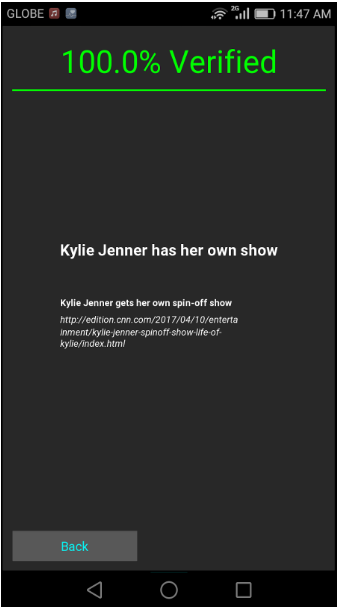
\includegraphics[width=2 in]{Capture}
		\end{center}
		\label{appui}
		\caption{The result interface of FactU.}
	\end{figure}

	\subsection{Program Flow}
	The application waits for an input IP Address of the server. The application (see Fig. \ref{appui}) then waits for an input statement or a URL from the user and sends it to the server. Upon receiving it on the server side, the string is preprocessed and is classified depending on whether it is a URL or a plain statement. If the input is a URL, a spider is deployed to the specific address and the title tag is extracted and parsed to be forwarded as a normal statement.
	
	A function then extracts the input's subject and the information from the database that contains the same subject is retrieved. All collected data are then passed on to the SSA module that compares the statement from each of the retrieved information from the database for a score that will used be later on used in the HMM module.
	
	The HMM module uses the similarity computed from the previous module to classify the input as verified or satiric. This result is then rendered in the front-end of the app that will display the result of SSA and HMM computations in the form a percentage. A short list of statements retrieved from the database with high similarity are provided as well. Each statement has a corresponding link for further reading.

	% RESULTS AND DISCUSSION
	\section{Results and Discussion}
	15 pairs of sentences were used as input for the three different approaches for Sentence Similarity Analysis (see Appendix \ref{appendix:survey}). A survey with 30 respondents was conducted to further assess these approaches. Both factors come up with a decision whether which approach is most suited for classifying news headlines before they are fed into the Hidden Markov Model for final computation of the result.
	
	NV space approach produces close results when it comes to statements that are assessed by the survey to be significantly the same. However, if the statements contain a related set of keywords but that have different meanings, the approach still gives a high similarity score despite survey respondents recognizing them as different.
	
	The Semantic and Word Order Similarity Approach was found to be more in line with the expected output based on the survey. Unfortunately, this approach generally gives relatively low scores since effectiveness is limited to short sentences.
	
	The triplet extraction approach outperformed the two other approaches (see Table \ref{tableb}) since it almost matched the expectation from the survey. Its disadvantage is that it requires both statements to have a subject, a verb, and an object to perform effectively.
	
	\begin{table}[h!]
	\caption{Comparison of 4 Different SSA Algorithms and Expected Result from Survey}
    	\begin{center}
    		\begin{tabular}{ |c|c|c|c|c|c| } 
    			\hline
    			& Triplet & NV-space & without IC & with IC & expected \\ 
    			\hline
    			1 & 0.781 & 0.827 & 0.682 & 0.596 & 0.633 \\ 
    			2 & 0.852 & 0.995 & 0.614 & 0.553 & 0.747 \\
    			3 & 0.744 & 0.706 & 0.572 & 0.525 & 0.633 \\ 
    			4 & 0.892 & 0.880 & 0.626 & 0.731 & 0.697 \\ 
    			5 & 0.889 & 0.868 & 0.351 & 0.512 & 0.810 \\ 
    			6 & 0.807 & 0.836 & 0.679 & 0.831 & 0.793 \\ 
    			7 & 0.212 & 0.707 & 0.317 & 0.417 & 0.200 \\ 
    			8 & 0.703 & 0.686 & 0.673 & 0.656 & 0.413 \\ 
    			9 & 0.510 & 0.789 & 0.336 & 0.499 & 0.550 \\ 
    			10 & 0.301 & 0.801 & 0.675 & 0.767 & 0.107 \\ 
    			11 & 0.534 & 0.864 & 0.694 & 0.695 & 0.323 \\ 
    			12 & 0.048 & 0.770 & 0.357 & 0.541 & 0.647 \\ 
    			13 & Error & 0.914 & 0.670 & 0.774 & 0.523 \\ 
    			14 & 0.639 & 0.938 & 0.673 & 0.755 & 0.693 \\ 
    			15 & 0.314 & 0.951 & 0.408 & 0.519 & 0.727 \\  
    			\hline
    		\end{tabular}
    		
    		\label{tableb}
    	\end{center}
    \end{table}
	45 sentences including URLs were also tested as input for the program to test its accuracy (see Appendix \ref{appendix:sentences}).
	
	Data gathered from testing resulted in an 77.78\% success rate. Some input resulted in `Insufficient Evidence' as an output because no entry from the database was able to pass the 75\% similarity threshold with the given input. On the other hand, some results were erroneous due to having a high similarity percentage with its corresponding database entry but also having a lot of other entries with significant similarities from the other classification (see Appendix \ref{appendix:data}). One of the test cases resulted into `Cannot access link' because the specific website does not let spiders crawl its documents.
	
	% CONCLUSION AND FUTURE WORK
	\section{Conclusion and Future Work}
	Web Crawling has its advanced uses and a wide array of techniques to play with to customize its functionality, although there is still no definite way of exhausting all relevant web pages to maximize its purpose. In this case, even though the data set already consisted of 5,000 news articles, some input statements still seem to have insufficient evidence.
	
	Out of the three approaches to calculate for a score to classify news statements, the Triplet-Extraction Approach, was found to produce the most realistic results when compared to the results received from the survey. Thus, it was considered the most appropriate approach to compute SSA values to be used for the HMM. Still, other approaches to sentence comparison may still improve the output of the program, and should be explored further.
	
	Although the Hidden Markov Model used in the study achieved 77.78\% accuracy, other computational models may be used to garner a more definite result. A bigger database with more information to calculate a better result might also be beneficial to future studies.
	
	
	
	% BIBLIOGRAPHY
	\bibliographystyle{IEEEtran}
	\bibliography{./cs190-ieee}
	
    % Activate the appendix
    % from now on sections are numerated with capital letters
    \appendices
    
    \section{Survey Questions}
    \label{appendix:survey}
    	\begin{enumerate}
		\item US seeks to cool tensions with EU over Gilbraltar \newline
		US wants to make peace with EU
		\item Ex-Trump adviser Carter Page met with russian intel operative in 2013\newline
		Carter Page had an appointment with a russian operative
		\item US working with china over North Korea \newline
		US teams up with China to fend off North Korea
		\item Russia could soon control a US oil company \newline
		An oil company in US will soon be owned by Russia
		\item Passenger plans legal action \newline
		Passenger wants to file a case
		\item Stem cells offer hope for autism \newline
		Stem cells may be the solution for autism
		\item Yahoo faces chinese dissidents' lawsuit \newline
		China prefers Yahoo over Gmail
		\item facebook targets 30,000 accounts in crackdown on fake news in France\newline
		Facebook showed fake news in France
		\item Zebra spotted roaming Riverside County Neighborhood \newline
		Zebra seen strolling around the park
		\item Turkey blocks wikipedia for not removing content \newline
		A man eating Turkey blocks wikipedia for content
		\item US attorney general vows crackdown on gang violence \newline
		Filipino attorney general vows to stop gang violence
		\item When it comes to Syria, the ball's in Trump's court \newline
		Trump controls matters regarding Syria
		\item Wanted: sociable hermit for Austrian cliffside retreat \newline
		Austrian cliffside retreat demands sociable introverts
		\item Syria chemical attack: Russia challenges Trump \newline
		Trump is challenged by Russia amidst Syria chemical attack
		\item Philippines: Duterte welcomes Chinese navy ship visit to Davao \newline
		Navy ship from China receive warm welcome from President Duterte
	\end{enumerate}
    
    \section{Test Data}
    \label{appendix:sentences}
    \begin{enumerate}
		\item US wants to make peace with EU
		\item Carter Page had an appointment with a russian operative
		\item US teams up with China to fend off North Korea
		\item An oil company in US will soon be owned by Russia
		\item Passenger wants to file a case
		\item Stem cells may be the solution for autism
		\item Trump is challenged by Russia amidst Syria chemical attack
		\item Kylie Jenner has her own show
		\item Zebra seen strolling around the Riverside County
		\item Facebook targets many accounts to help keep track of fake news
		\item Attorney general from US vows to handle gang violence
		\item President Rodrigo Duterte warmly welcomes navy ship from China
		\item Wikipedia was blocked by Turkey for not pulling out information
		\item Ex-Trump Adviser Met With A Russian Spy
		\item Arrest of foreigners increase under Trump regime
		\item http://www.complex.com/pop-culture/2017/04/kylie-jenner-getting-her-own-show-life-of-kylie
		\item https://news.vice.com/story/russia-oil-rosneft-infrastructure
		\item https://www.cnet.com/au/news/facebook-targets-coordinated-campaigns-spreading-fake-news/
		\item http://nypost.com/2017/04/06/russia-challenges-trump-after-syria-chemical-attack/
		\item http://nypost.com/2017/04/14/solar-powered-device-turns-air-into-drinkable-water/
		\item Britney Spears to be taken care by African child
		\item www.slate.com/articles/news-and-politics/low-concept/2007/10/save-the-celebrity-children.html
		\item Glenn Beck calls for help after eating halal pizza
		\item http://www.visajourney.com/forums/topic/413120-glenn-beck-calls-911-after-accidentally-eating-halal-pizza/
		\item Palin licks Frozen Flagpole
		\item https://theintellectualist.co/sarah-palin-licks-frozen-flagpole-in-iowa-gets-stuck/
		\item Landfill was named 'Obama' in North Dakota
		\item http://www.a-cnn.com/index.php/articles/item/1322-north-dakota-names-landfill-after-obama
		\item Barry Manilow is a homosexual
		\item https://www.theguardian.com/music/2017/apr/05/barry-manilow-reveals-he-is-gay
		\item Safest place during tornado is in my arms
		\item brain scan can show your dreams
		\item http://www.wired.co.uk/article/neuroscience-of-dreaming-consciousness
		\item North Korea kills nuclear scientist
		\item https://www.democraticunderground.com/1016184083
		\item Trump shows Son how to hunt in zoo
		\item http://www.scoopnest.com/user/TheOnion/854742206376181761
		\item Scorpion stings passenger while in flight
		\item UP bestows honorary degree on Aquino
		\item Sky got the contract for Easter Week TV
		\item Duterte is a murderer
		\item Duterte is dead
		\item Philippines bans pork
		\item Dinosaur found in Palawan
		\item Oregano can kill cancer
	\end{enumerate}
	\newpage
    \section{Test Data Results}
    \label{appendix:data}
    \begin{table}[h!]
    \caption{A comparison of Computed Scores and Expected Output}
    	\begin{center}
    		\begin{tabular}{ | c | c | c |} 
    			\hline
    			Sentence & Computed Result & Expected Result\\
    			\hline
    			1 & 87.08 Verified & Verified\\
    			2 & 81.03 Verified & Verified\\
    			3 & 78.76 Verified & Verified\\
    			4 & 83.20 Verified & Verified\\
    			5 & 81.86 Verified & Verified\\
    			6 & 80.66 Verified & Verified\\
    			7 & 86.82 Verified & Verified\\
    			8 & 100.0 Verified & Verified\\
    			9 & Insufficient Evidence & Verified\\
    			10 & 90.57 Verified & Verified\\
    			11 & 76.48 Verified & Verified\\
    			12 & Insufficient Evidence & Verified\\
    			13 & 80.21 Verified & Verified\\
    			14 & Insufficient Evidence & Verified\\
    			15 & 82.50 Verified & Verified\\
    			16 & 85.00 Verified & Verified\\
    			17 & 90.97 Verified & Verified\\
    			18 & 77.84 Verified & Verified\\
    			19 & 86.90 Verified & Verified\\
    			20 & 94.20 Verified & Verified\\
    			21 & 82.64 Satiric & Satiric\\
    			22 & 76.67 Satiric & Satiric\\
    			23 & 95.10 Satiric & Satiric\\
    			24 & 100.0 Satiric & Satiric\\
    			25 & 85.00 Satiric & Satiric\\
    			26 & 100.0 Satiric & Satiric\\
    			27 & 75.00 Satiric & Satiric\\
    			28 & 100.0 Satiric & Satiric\\
    			29 & 81.91 Satiric & Satiric\\
    			30 & 100.0 Satiric & Satiric\\
    			31 & 100.0 Satiric & Satiric\\
    			32 & 75.49 Verified & Satiric\\
    			33 & 78.81 Satiric & Satiric\\
    			34 & 88.39 Verified & Satiric\\
    			35 & 80.92 Verified & Satiric\\
    			36 & 88.21 Verified & Satiric\\
    			37 & Cannot Access Link & Satiric\\
    			38 & 77.82 Satiric & Satiric\\
    			39 & 92.50 Satiric & Satiric\\
    			40 & 89.20 Satiric & Satiric\\
    			41 & 85.93 Verified & Insufficient Evidence\\
    			42 & Insufficient Evidence & Insufficient Evidence\\
    			43 & 83.89 Verified & Insufficient Evidence \\
    			44 & Insufficient Evidence & Insufficient Evidence \\
    			45 & Insufficient Evidence & Insufficient Evidence \\
    			\hline
    		\end{tabular}
    		\label{tablec}
    	\end{center}
	\end{table}
\end{document}
